\documentclass[../../main.tex]{subfiles}
\begin{document}
% As stated in section \ref{sec:ProblemDescription}, the main goal of the project has been to apply knowledge of embedded C and VHDL programming to interface motor encoders in a pan-tilt system, and implement a framework for a discrete controller which allows the robotic system to be manipulated to given positions. Using knowledge gained from the concurrent control systems course, different controller designs and design methods should be assessed, in an attempt to meet the overall system specifications presented in table \ref{tab:performanceSpec}. Simulation results should be compared to results obtained from testing the physical system.

During the project, choices have been made with regards to design of controllers and implementation on the given devices. Some of these choices, both due to inexperience in the disciplines and due to initial project conditions, have proved to be inadequate towards meeting the system response requirements decided by the project group in section \ref{sec:Requirements}. In this section the results as well as the choices and alternatives will be discussed.

\subsection{Evaluating Performance}

Looking at table \ref{tab:controller_data} it is seen that the specifications established in section \ref{sec:Requirements} have not been completely met by any of the implemented controllers. In this regard, it must be acknowledged that none of the simulations meet all the specifications either. A more experienced control engineer might have settled on less strict requirements.
%In hindsight these specifications, especially the one about settling time, have probably been slightly unrealistic from the beginning. 
Over all it has been possible to achieve performances which are not too dissimilar from those that were found through simulation. It is likely that manually tuning the parameters of the controllers, based on the values presented in this report, could improve the performance. Had more time been available, this would have been interesting to study further. After all, one of the main advantages of the PID-controller is the fact that it is simple to tune. 

Initially, it was expected that the cascaded controller design would yield better performance when implemented compared to a single controller, since it theoretically offers better rejection towards noise. However, with the chosen designs the cascaded controllers actually performed worse than the single controller designs in both simulations and implementation. This is likely because the velocity controllers should have been designed to have a faster response. For cascade control to make sense, the dynamics of the inner loop should be at least five times faster than the dynamics of the outer loop. Furthermore, the velocity controller should have had a high gain to limit disturbances. Had these requirement been properly met in designing the velocity controllers, the cascade control performance may have been better. It should also be mentioned that it has later been found that using a full PID in an inner loop is unconventional. Usually either PI or just P control is used for inner loops \cite{}.
%Due to the fact that the control signals on the physical setup is limited to \SI{\pm 12}{\volt}, the controllers were designed in a way that attempted to minimise how much the controls signal saturates. At the same time, the design and tuning of the cascaded controller also becomes more complex, since there are more zeros and pole to consider, and more parameters to tune. 
It was also found that the cascaded controller which relied purely on the mathematical model of the system performed drastically worse than the one which made use of the Ziegler-Nichols tuning method. This is not unexpected, since it is acknowledged that several imperfections in the mathematical model of the pan-tilt system exist. Therefore a heuristic approach such as the Ziegler-Nichols is likely to yield equally good or better results as the model based approach. Considering figures \ref{fig:StepTiltPos}, \ref{fig:StepVelZN} and \ref{fig:Cascade_ZN_tilt} it can be seen that, the response from the physical system is actually quite close to the simulated response of the tilt motor. This indicates that the mathematical model of the tilt motor is somewhat accurate. The big deviations which are seen in figure \ref{fig:StepVelModel} and \ref{fig:cascade_model_tilt} are likely caused by another issue which is discussed later in section \ref{subsec:TheFiltering}. Figure \ref{fig:StepPanPos} and \ref{fig:cascade_ZN_pan} shows that a lot more deviation is found for the model of the pan motor. This makes sense since the parameters, which are found experimentally in section \ref{subsec:motorParameters}, are based solely on the tilt motor. If disassembling the pan-tilt system was allowed, it would be interesting to perform similar tests to determine the parameters of the pan motor. From looking at the two figures it also appears that the pan motor generally has a slower response than the model predicts, which among other things could indicate that the estimation of the inertia of the pan motor is too low. This is likely to be true since the simplifications, introduced in section \ref{subsec:motorParameters}, will yield a slightly lower result for the inertia especially for the pan motor.


% non linear relation between duty cycle and voltage.

% why does the tilt position controller based on model do the best? - something about the best model representation. It seems like the actual pan motor has more inertia than what is modeled. The cascade seems to be worse. Why? because of the poor velocity control.
%discuss the fact that the requirements are not met. Could we have met them? Probably not with the saturation and such. Given enough power the response 
%Model deviations and non-linearities
% include the open loop step responses


\subsection{Encoder Accuracy and Resolution}
As the angular velocity is deduced from the encoder output, the performance of the PID-controllers and the accuracy of the encoders is closely linked. As seen in figure \ref{fig:VelocityTilt} the measured velocity response is very noise. The accuracy of the motor encoder has been recognised as one of the possible sources of this noise. 
% As described in section \ref{subsec:SystemImplemtationFPGA} the encoder provided with each motor only has a resolution of 360 counts for a full revolution. At 
The accuracy of the motor encoder is inadequate, as the time between encoder edges at a constant angular velocity is not constant. Table \ref{tab:EncoderDifferenceBetweenEdges} shows the time period between consecutive encoder edges. The data is sampled from the tilt motor encoder, over a period of 14 encoder edges, while a constant voltage is applied to the motor. It is acknowledged that the angular velocity is uneven through one revolution of the tilt frame. It is presumed that this velocity variance can be neglected due to the short time frame of the 14 edges compared to the 1080 for a full revolution. 
The percentage increase from the minimum time period to the maximum time period is \SI{59.6}{\percent}.
% \begin{equation} \label{eq:PercantageIncreaseEncoderProblem}
%     \Delta t_{max} = \frac{1.66 - 1.04}{1.04} \cdot 100 = \SI{59.6}{\percent} 
% \end{equation}

The difference is significant. In this section the consequences of this encoder behaviour and the fact that little is done to compensate for the behaviour and what could have been done is discussed.

\begin{table}[H]
    \centering
    \begin{tabular}{c c c c c c c c c c c c c c c}
         \multicolumn{13}{c}{Time period (ms)} \\ \hline
         
         1.28 &
         1.52 &
         1.42 &
         1.4  &
         1.34 &
         1.66 &
         1.04 &
         1.66 &
         1.26 &
         1.38 &
         1.34 &
         1.6  &
         1.22 
       
    \end{tabular}
    \caption{The time period between encoder edges measured in milliseconds with a duty cycle of \SI{77}{\percent}.}
    \label{tab:EncoderDifferenceBetweenEdges}
\end{table}

One way to compensate for the inconsistency would be to group four edges of the encoder signals into one count. This would result in percentually less variance between counts than what is experienced with the current implementation. With this modification the resolution of the encoder module would be 90 counts per revolution, four times lower than the original resolution, which is not desired. This would introduce other problems for the PID-controllers implemented, as the rate at which new data is available would decrease.
%Also it is possible that the variance can be attributed to the inaccuracies of the oscilloscope used to measure. With this modification the resolution of the encoder module would be 90 counts per revolution, four times lower than the original resolution, which is not desired. This would introduce other problems for the PID-controllers implemented, as the rate at which new data is available would decrease.

%As mentioned in section \ref{subsec:SystemImplemtationFPGA} there are two ways to determine the speed from the encoder readings. The issue with the inconsistent distance between encoder counts is relevant for both methods. 

As mentioned in section \ref{subsec:SystemImplemtationFPGA}, another way of determining the angular velocity would be to count encoder edges in a constant time period. Possibly this method compensates for the inaccuracy of the motor encoders better than the method utilised, as the variance in the time between encoder edges becomes less significant when the amount of encoder edges between a time period is high. 

Currently, the PID-controllers sample the Speed module every \SI{1}{\milli \second}. This requires the Speed module on the FPGA to update the speed value with a frequency of at least \SI{1}{\kilo\hertz}. With a resolution of the motor encoder at 1080 encoder counts for one revolution and one revolution taking approximately 5 seconds for the tilt frame at its slowest speed, this yields an average of 0.2 encoder counts per sample. This would not be adequate for calculating the angular velocity. 

% The tilt frame at the slowest speed however, takes approximately 5 seconds for a full revolution. With 1080 encoder counts for one rotation, this would with a constant time period of $\SI{ 1 }{ \milli \second } $, yield 2-3 counts per time period. A resolution far to low to be utilised for providing feedback to any controller.

% To go around the issue of variance in between encoder edges, the option to count encoder edges in a constant time period could be used. With this method, small differences in the time between encoder edges would not have as much significance, when the number of encoder counts in the time period is relatively high. Generally the variation is less significant when it compares to a higher value.

% Currently at the slowest speed at which the tilt frame is able to continuously rotate, the tilt frame takes approximately 5 seconds for a full revolution. This yields 1.66 seconds per revolution of the motor. With an encoder resolution of 360 ticks per revolution the amount of encoder counts per second would be $360 / 1.66 \approx 217 $. With a constant time period of $\SI{ 10 }{ \milli \second } $ this yields 2-3 counts per time period. A resolution far to low to be utilised for feedback. Maintaining this motor speed the speed measured would most of the time read the value 2 and occasionally 3. A jump from 2 to 3 corresponds to a \SI{50}{\percent} increase while the other way would result in a \SI{33}{\percent} decrease, changes in readings that when used as feedback would be to much for the PID-controllers to handle.

% An option to mitigate the sudden changes in encoder readings would be be to constantly compute a moving average of the encoder readings, which would smooth out the differences between the readings. However this would come at the cost of latency. A change in speed would not immediately be read by the result of the moving average, instead being delayed. This delay would introduce problems on its own for the PID-controllers. 

The optimal solution would probably be to replace the current motor encoders with encoders with much higher resolution and better precision. Encoders with resolution in the 1000- and 10000-range are easily available. An encoder with better resolution would make it more viable to count encoder edges within a constant time period, even at the lowest possible speed.

% Such encoders would make it more viable to perform computation of speed with a constant time period. With the slowest possible speed of the motors at about 5 seconds per revolution of the frame, yielding 1.66 seconds per revolution of the motor and an encoder resolution of 4096 encoder counts per revolution the amount of encoder counts per second would be $4096 / 1.66 \approx 2467$.
% For a constant time period of $\SI{ 1 }{ \milli \second }$, this would only yield 2-3 encoder counts per time period. Far too low for reliable operation. With a constant time period of $\SI{ 10 }{ \milli \second }$, though this would yield 24-25 encoder counts, a more reliable resolution at the expense of a lower sampling rate, that probably could be tolerated.

%Poisition, step response

\subsubsection*{The Filtering} \label{subsec:TheFiltering}
As described in section \ref{subsec:SystemImplementationMicroController}, filtering the feedback data was at first not assumed important to achieve good system response. With the very noisy velocity feedback data presented in figure \ref{fig:StepVelZN} and \ref{fig:StepVelModel} however, it is apparent that filtering is particularly important in this system. In neither of the figures does the system converge to the reference even though integral terms are implemented to correct this. Simulations, presented in figure \ref{fig:StepResponsAddedNoise} and \ref{fig:StepResponsAddedNoiseAndFilter}, indicate that the deviation from the reference could be due to noise affecting the derivative term.

It is wanted to evaluate the effect of the implemented fifth order FIR filter. In figure \ref{fig:FilteredStepRespons5Order}, the implemented filter, described in section \ref{subsec:SystemImplementationMicroController}, is applied to the raw velocity feedback data. The figure shows a filtered but noisy signal and from the tests section \ref{sec:Test}, it is obvious that the controller does not reach the reference.

%In figure \ref{fig:FilteredStepRespons5Order} the low pass FIR filter equation \ref{eq:derivative_filter}, is applied to the raw velocity feedback data.

Trying to understand how noise affects the response of the system, a step response is simulated where a high frequency sine wave is imposed on the feedback signal to emulate the noise. The simulation is shown in figure \ref{fig:StepResponsAddedNoise} and is based on the setup used for the pole placement based velocity controller test described in section \ref{subsec:testControllerDesign}.

\begin{figure}[H]
     \centering
     \begin{subfigure}[b]{0.49\textwidth}
         \centering
    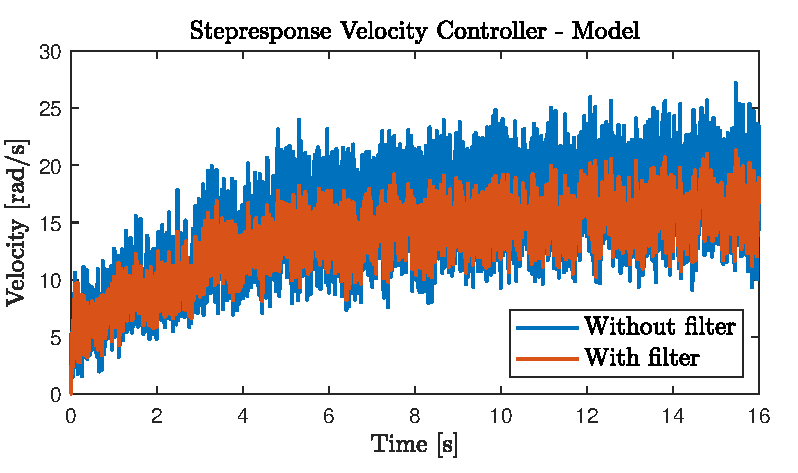
\includegraphics[width=\textwidth]{Sections/Miscellaneous/Images/FilteredStepRespons5Order.pdf}
    \caption{Fifth order FIR filter applied to raw velocity feedback data}
    \label{fig:FilteredStepRespons5Order}
     \end{subfigure}
     \hfill
     \begin{subfigure}[b]{0.49\textwidth}
         \centering
         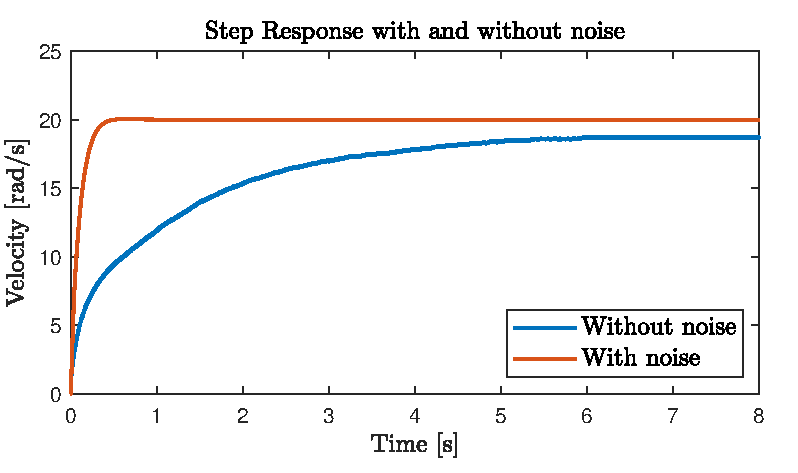
\includegraphics[width=\textwidth]{Sections/Miscellaneous/Images/StepResponsAddedNoise.pdf}
         \caption{Simulation of the system with added noise.}
         \label{fig:StepResponsAddedNoise}
     \end{subfigure}
        \caption{Simulation results when applying a fifth order FIR to the velocity feedback.}
        \label{fig:FilterDiskussionImplementedFilter}
\end{figure}
From figure \ref{fig:StepResponsAddedNoise} it is clear that the noise increases the rise time and lowers the value that the response converges towards. On figure \ref{fig:StepResponsAddedNoiseAndFilter} a filter is implemented on the derivative term with transfer function $H(s) = \frac{5}{5+s}$. With the noise components at higher frequencies being dampened, the derivative term performs much better allowing for faster response and the system almost converging towards the reference at \SI{20}{\radian \per \second}. This emphasises that it would have been favourable to put more time into deliberately designing a filter, in order to accomplish a response with less error when noise is present.

\begin{figure}[H]
     \centering
     \begin{subfigure}[b]{0.49\textwidth}
         \centering
    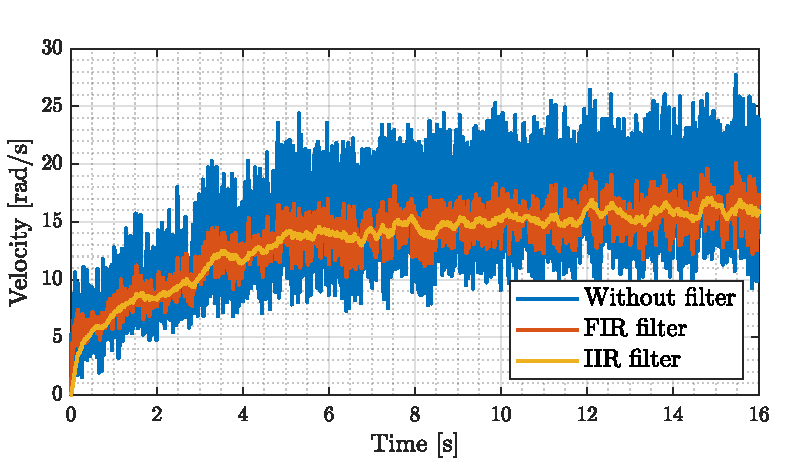
\includegraphics[width=\textwidth]{Sections/Miscellaneous/Images/FilteredStepRespons20Order.pdf}
    \caption{20th order FIR filter and a first order IIR filter applied to raw velocity feedback data.}
    \label{fig:FilteredStepRespons20Order}
     \end{subfigure}
     \hfill
     \begin{subfigure}[b]{0.49\textwidth}
         \centering
         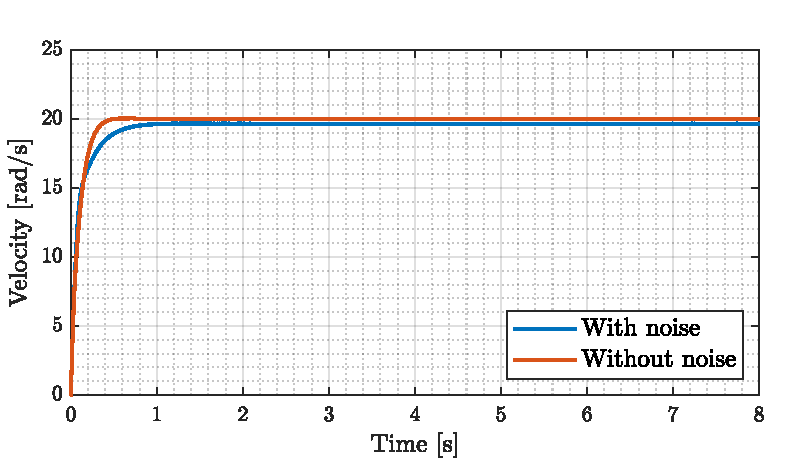
\includegraphics[width=\textwidth]{Sections/Miscellaneous/Images/StepResponsAddedNoiseAndFilter.pdf}
         \caption{Simulation of the system with added noise and filter on the derivative term.}
         \label{fig:StepResponsAddedNoiseAndFilter}
     \end{subfigure}
        \caption{Simulation results when applying FIR and IIR filters to the raw velocity feedback data.}
        \label{fig:FilterDiskussionImplementedFilter20}
\end{figure}
On figure \ref{fig:FilteredStepRespons20Order} a $20^{th}$ order filter is applied to the raw velocity feedback data. Even though the amplitude of the data is even smaller than with a fifth order filter, it is still noisy. A test would be necessary to see if the response would meet the chosen requirements. The figure also shows that using an infinite impulse response filter, substantially better noise reduction can be achieved using only a first order filter. Implementing an IIR filter may have been beneficial to achieve better performance.

\subsection*{Using built-in hardware in the Tiva launchpad}
The project description states that the FPGA must be used for interfacing with the pan-tilt system, while the microcontroller must handle the user input and that these two development kits must communicate to each other through SPI. However the processing power available on the microcontroller alone or the amount of logic blocks available on the FPGA alone far exceeds the requirements by the scope of the project. Therefore it is possible to implement the project on just one of the devices. It is clear that the project is constructed in this way to encompass all disciplines taught on the semester. However, it is also wanted to clarify that had this project been ordered by an employer, it would have been implemented on just one of the devices. A typical choice could be to implement the system on the microcontroller. The microcontroller features peripherals implemented in physical hardware, for handling PWM and getting position and velocity readings from an encoder. As these are implemented in hardware in the microcontroller and since new data can be flagged by interrupts, eliminating the need for the microcontroller to poll the data, the microcontroller still has plenty of processing power left while handling all the tasks that the FPGA handles. The use of the microcontroller as interface to the encoder would also eliminate the need for additional SPI functionality.
%\subsection*{Reset from both directions}

% \subsection*{Test Methods}
% It is noted that it would have beneficial to plot the control signal along with the step responses of all tests. This would have made it easier to comprehend and conclude on the behaviour of the responses. 
% As concluded in the tests section \ref{sec:Test}, there is a difference between the simulated and the implemented response of the controllers. A comparison between the physical step response and the model can be seen on figure \ref{fig:Mes_vs_siml}. The two responses resembles each other fairly well, though if examined further it is seen that there is a difference in the steady state of around 2-3 \si{rad/s}. Also worth noticing is the undulation in the actual response, making it apparent that some parameters are not taken into account or flaws in the estimation of parameters. 
% \begin{figure}
%     \centering
%     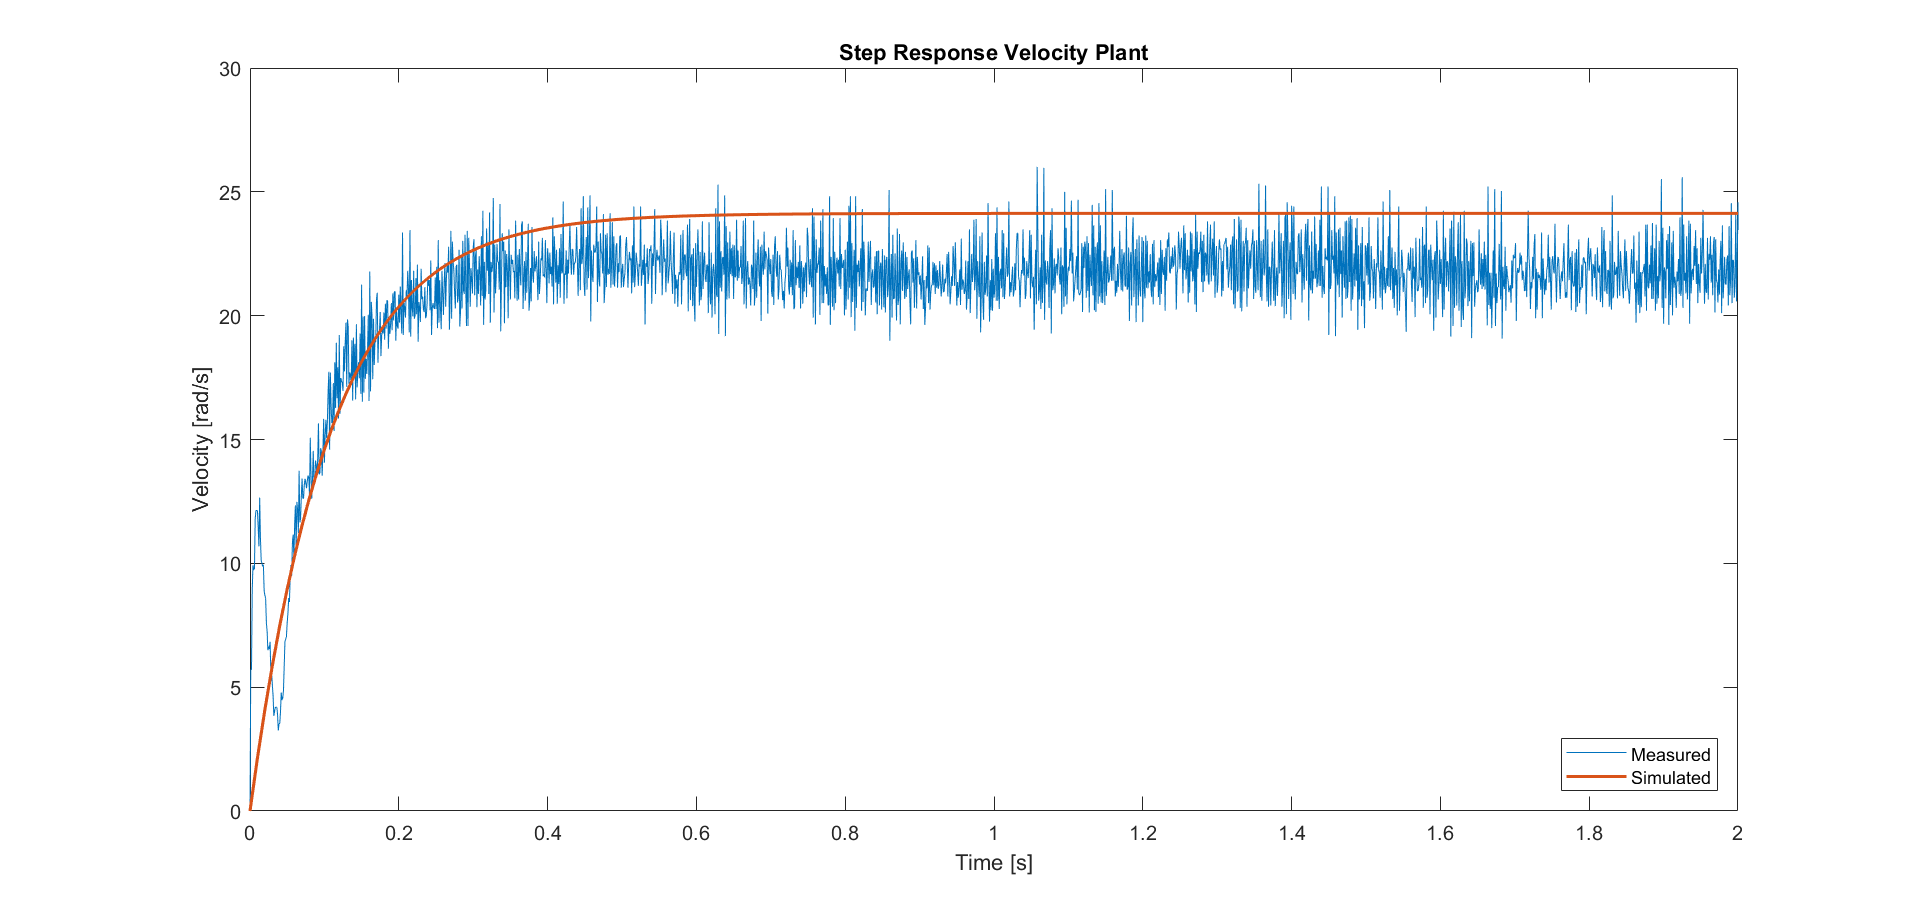
\includegraphics[width = 0.9 \textwidth]{Sections/Miscellaneous/Images/velocityPlantMes_vs_Sim.png}
%     \caption{Measured and simulated system response.}
%     \label{fig:Mes_vs_siml}
% \end{figure}



\subsection*{Modern Control}
As mentioned in section \ref{sec:Analysis} other control techniques than the PID-controller are available. Modern control techniques uses state feedback to control the system and requires an immense knowledge of the system in question, hence the PID-control was prefered for the project. However it is of great interest to examine the possibility of using modern techniques, enabling the possibility of using observers and estimating otherwise unknown states such as the current. An integral controller with an observer and anti-windup as illustrated on figure \ref{fig:Integral_Observer_Diagram} could be advantageous to implement. The aforementioned constellation introduces four gains to be found namely the feedback gain, $F$, the integral gain, $F_I$, the observer gain, $L$, and anti-windup gain, $M$. The controller leaves a lot of customizability, in the sense that the gains can be tuned to achieve the wanted response of the system, however at the cost of great complexity compared to the PID-controller.


\end{document}